\section{Tuesday, January 16th}
\subsection{Communication}
We work with the following model:
\begin{figure}[H]
    \centering
    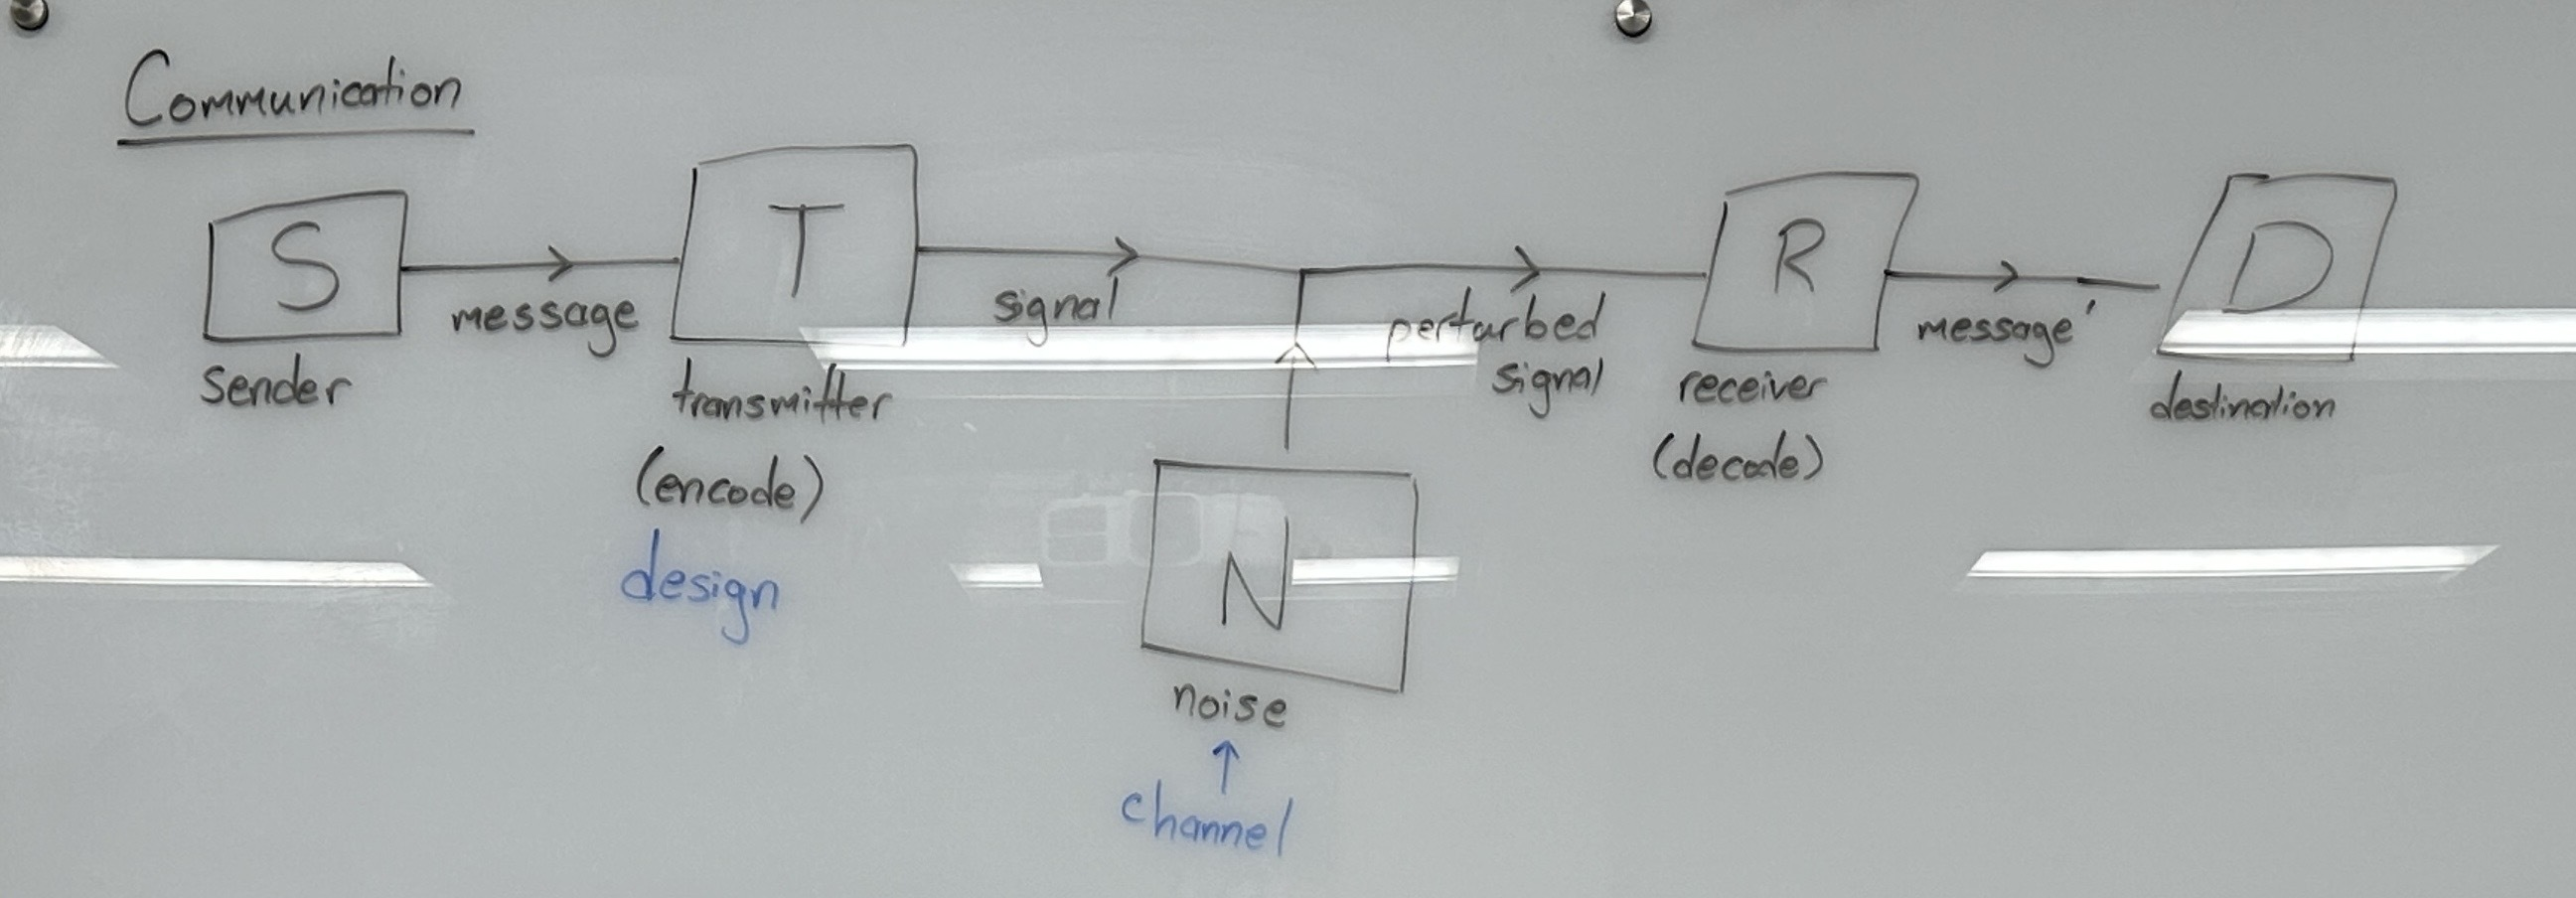
\includegraphics[scale=0.18]{lectures/wk1/img/communication.png}
    % \caption{Caption}
    % \label{fig:enter-label}
\end{figure}

which consists of the following entities:
\begin{itemize}
    \item Sender: you
    \item Message: What you want to send
    \item Signal: What you actually sent
    \item Transmitter: a function that encodes messages to signals
        \begin{itemize}
            \item This is a design question: we want to make it so that the perturbed signal can be decoded with minimal error
        \end{itemize}
    \item Source of Noise: different depending on how the channel works, but fixed to the type of channel
    \item Perturbed signal: signal + noise
    \item Receiver: they decode the perturbed signal to get message' which is then sent to the destination 
\end{itemize}

\subsection{Channel Capacity}
\begin{defn}{Channel Capacity}
$\max$ over possible encodings of the rate at which we can send information (messages) with low error.

What is the rate that you can send signals?
\end{defn}

\textit{Statistical} Information: Does not care about content of the message — instead: How many encodings can be represented?\\
This is as opposed to being length-agnostic where panther has more info than animal.

Problem: observe \( Y=y \), estimate the original \( X \) given \( Y=y \) related by conditional distribution of \( X|Y=y \)

\begin{itemize}
    \item Prior: \( P(X = x) \)
    \item Posterior: \( P(X = x | Y = y) \)
    \item Likelihood: \( P(Y = y | X = x) \)
\end{itemize}

Posterior \( \propto \) Likelihood \( \times \) prior, where alpha means proportional to (there’s some factor in the denominator that we are not caring about).

Information: The reduction of uncertainty regarding what was sent given what was received.
\begin{itemize}
    \item Regarding an unknown after an observation
\end{itemize}

But now we need to think how do we measure uncertainty in \( X \), \( H(X) \)?\\
We say \( U[X]=U(p) \) is a functional:
\begin{itemize}
    \item \( f \rightarrow I[f] \) is equivalent to \( \int f \)
\end{itemize}
Then we can think about the uncertainty in \( X \) after an observation, \( H(X | Y=y) \).\\
Finally we could average over all possible received messages to define:
\[ I(X; Y=y) = H(X) - H(X | Y=y) \]

We want a function that is a measure of uncertainty that is symmetric/invariant over all possible choices of labels (i.e. random variables).

\subsection{Extrinsic vs Intrinsic Measures}
Extrinsic measures: Depends on a realization of probability space (i.e. variance). You are measurable.
\begin{itemize}
    \item Depends on how you label your outcomes.
    \begin{itemize}
        \item This is useful if you lost your keys in 1 of 3 places and want to know the name of the place where you lost your keys
    \end{itemize}
    \item Traditional Statistics
    \item Functions of, expectation of random variables.
\end{itemize}

Intrinsic measures: Information Theory is the best example of this with uncertainty.
\begin{itemize}
    \item Depends only on the probability space, the set of outcomes, list of probabilities. Example: \( p=[p_1, p_2, \ldots, p_\Omega] \)
    \item \( U(p) \) is permutation invariant. That is, \( U[p]=U[p'] \).
    \begin{itemize}
        \item This is good if you want to know \( P[\text{err} | b] \) and don’t want the answer to be dependent on ‘a’ being before ‘b’
        \item Also makes sure the same statement in English vs French vs etc. gives the same entropy.
    \end{itemize}
\end{itemize}

\subsubsection{When does Intrinsic matter more than extrinsic?}
\begin{itemize}
    \item Suppose that \( X \) is a random variable with finitely many discrete \& distinct outcomes, which takes on integers \( \geq -1 \).
    \item Also suppose we can get exact answers to questions of the form: is \( X > \alpha \) for any \( \alpha \).
    \item How many answers do I need on average to know the value of \( X \).
\end{itemize}

You can scale the labels (dilate the graph out horizontally) which would change extrinsic measures but not intrinsic measures. \( \text{Var}(aX) \neq \text{Var}(X) \) but our Intrinsic question above does not care.
